\documentclass[9pt,twoside]{pnas-new}

\templatetype{pnassupportinginfo}

% The SI format has no manuscript line-number headers. Clearing the inherited
% draft headers also keeps the 2018 SI style compatible with pnas-new v1.46.
\fancyhead{}

\usepackage{siunitx}

\graphicspath{{../supplement/figures/}{../figures/}}

\newcommand{\coTwo}{CO$_2$}
\newcommand{\todo}[1]{\textbf{[TODO: #1]}}

% The official PNAS SI style suppresses ordinary section labels. These local
% wrappers retain its typography while printing the requested SI hierarchy.
\newcommand{\SISection}[1]{%
  \refstepcounter{section}%
  \section*{\thesection.\ #1}%
  \addcontentsline{toc}{section}{\protect\numberline{\thesection}#1}%
}
\newcommand{\SISubsection}[1]{%
  \refstepcounter{subsection}%
  \subsection*{\thesubsection.\ #1}%
  \addcontentsline{toc}{subsection}{\protect\numberline{\thesubsection}#1}%
}

\title{End-to-End Uncertainty Quantification of Geologic \coTwo{} Storage in Faulted Reservoirs}
\author{Shaowen Mao, Llu\'{\i}s Sal\'o-Salgado, Hannah Lu, Patricia Ascanio-Pellon, Christie M. Rogers, Nathan W. Harkins, Rodrick D. Myers, Lisa Lun, and Ruben Juanes}
\correspondingauthor{Corresponding author: Ruben Juanes. Email: juanes@mit.edu}

% The complete nine-author list does not fit in the official SI running footer.
% Keep it on the title page and use the conventional short running author.
\fancyfoot[LO,RE]{\bfseries\sffamily Mao et al.}

\begin{document}

% The official template instruction page is intentionally omitted from the
% compiled manuscript-ready SI PDF.
\maketitle
\SItext

This Supporting Information provides the complete methodological description
and supporting diagnostics for the study. Its six sections follow the
end-to-end workflow from the offshore Texas field case and geologic design,
through local fault-core modeling and property upscaling, to full-fault field
construction, field-scale simulation, and uncertainty analysis. The main
manuscript retains the study assumptions needed to interpret the results,
while implementation details and validation procedures are consolidated here.
Data and software are deposited separately and cited through the manuscript's
data-availability statement.

% Start the six-stage SI hierarchy after the unnumbered title-page material.
\setcounter{section}{0}
\setcounter{subsection}{0}
\renewcommand{\thesection}{\arabic{section}}
\renewcommand{\thesubsection}{\Alph{subsection}}

% !TEX root = ../supporting_information.tex

\SISection{Offshore Texas Field Case and Geologic Uncertainty}
\label{sec:si-field-case-geologic-uncertainty}

\SISubsection{Geologic model}

The Gulf Coast of Texas has been considered a promising region for geologic \coTwo{} storage due to its thick, laterally extensive, and regionally continuous Miocene sandstones. We focus on the Miocene section within the Texas State Waters, which is an attractive offshore alternative to onshore storage. The setting








The geologic setting consists of



The field-scale model represents an offshore Texas storage setting with
approximately two million grid cells and a three-dimensional growth fault that
offsets the storage interval and partially offsets the top seal.

\todo{Insert the final field-model dimensions, boundary conditions, spatial
resolution, and geologic rationale.}

\SISubsection{Fault-region discretization and throw windows}

The portion of the fault intersecting the top-seal system is divided into six
throw windows along dip and 87 slices along strike. Local juxtaposition
therefore varies among windows, and each full-fault property realization
contains $6\times87=522$ fault elements. Layer order and thickness are stored
separately for the footwall and hanging wall of every window so that the
geology-specific stratigraphy and fault-property files can be paired and
validated before reservoir simulation.

\todo{Provide the final window boundaries, discretization dimensions, and
their geologic rationale.}

\SISubsection{Geologic scenario design}

The prescribed design contains six layer-thickness structures spanning low,
medium, and high sand proportions with uniform and nonuniform thickness. Each
structure is combined factorially with three faulting depths, three
clay-volume fractions in sand-rich units, and three clay-volume fractions in
clay-rich units, producing
\begin{equation}
  6\times3\times3\times3=162
\end{equation}
geologic scenarios. Every scenario has equal design weight. The ensemble is
therefore suitable for controlled comparisons across the prescribed
fault--seal space, but its frequencies are not interpreted as calibrated
field occurrence probabilities.

\todo{Tabulate the final factor levels, units, and the mapping from geology
identifiers to the complete factorial design.}

% !TEX root = ../supporting_information.tex

\SISection{Stochastic modeling of local 3D fault-core architectures}
\label{sec:si-local-fault-core-modeling}

\SISubsection{PREDICT inputs and stochastic realization generation}

For each geology and throw window, PREDICT generates 2,000 accepted stochastic
fault-core realizations conditioned on local stratigraphy, fault throw, and
the prescribed geologic parameters. Adjacent units of the same lithology are
collapsed before fault-core generation so that artificial boundaries between
equivalent neighboring units do not create additional smear sources. Each
accepted realization retains its fine-scale material architecture and one
actual joint permeability vector $(k_{xx},k_{yy},k_{zz})$. The three
permeability components are never selected independently.

The PREDICT model formulation, stochastic fault-core construction, and
property-upscaling framework are described by Sal\'o-Salgado et
al.~\cite{SaloSalgado2023,SaloSalgado2025}; the public implementation and
examples are available at \url{https://github.com/lsalo/predict}. We therefore
document only the study-specific ensemble design and convergence assessment
here.

\refstepcounter{table}
\label{tab:si-predict-ensemble}
\noindent\textbf{Table \thetable.} Summary of the PREDICT ensemble used by the
full-fault workflow. Replace provisional entries and add the final
scenario-level parameter values before submission.
\begin{center}
  \begin{tabular}{@{}ll@{}}
    \toprule
    Item & Current design \\
    \midrule
    Geologic scenarios & 162 \\
    Throw windows per geology & 6 \\
    PREDICT realizations per window & 2000 \\
    Permeability components retained jointly & $k_{xx}$, $k_{yy}$, $k_{zz}$ \\
    Layer representation & Adjacent same-material units collapsed \\
    \bottomrule
  \end{tabular}
\end{center}

\SISubsection{PREDICT convergence assessment}

We assess how many PREDICT realizations are needed to obtain stable
distributions of upscaled fault permeability. The assessment uses one
fixed-stratigraphy scenario from the Texas offshore case. The scenario contains six
throw windows, and we assess convergence separately for each window using
independent Monte Carlo ensembles.

We first generate three independent large ensembles (20,000 PREDICT realizations) for each window. Note that we do not treat any of these finite ensembles as the exact or true permeability distribution. Instead, we compare the permeability distribution of three large ensembles pairwise by calculating the distance between each pair of distributions, and then take the median of the three distances to define a reference floor. The reference floor is typically very small because of the large number of realizations in each ensemble, so it can be used to evaluate whether smaller ensembles with fewer PREDICT realizations are converging to a stable permeability distribution. The distance metrics are described in the next paragraph.

We then perform PREDICT simulations with
fewer realizations to assess convergence for each window. We test
$N=\{20,50,100,200,300,400,500,750,1000,1500,2000\}$. We
generate 30 independent repeated ensembles for each $N$. We compare each ensemble with all three large ensembles with 20,000 realizations pairwise, calculating the distance between each pair of permeability distributions. Each ensemble has three distances to the three large ensembles, and we use the median of the three distances for convergence analysis. The distance between two permeability distributions is calculated in $\log_{10}(k\,[\mathrm{mD}])$ space using two distribution-distance metrics: (1) mean absolute error (MAE) between histogram probabilities on 24 common bins spanning $[-7,3]$ and (2) the exact empirical one-dimensional Wasserstein-1 distance computed from the unbinned samples. A larger distance indicates that the two distributions are more different.

To assess whether a common ensemble size provides consistent convergence
across all throw windows and permeability components, we pool the distances
after normalizing each by the reference floor for its window, component, and
metric. Figure~\ref{fig:si-predict-convergence} shows how these pooled
normalized distances vary with $N$. The median normalized distance decreases
monotonically with increasing $N$. Across the 18 window--component
combinations, log--log fits have median slopes of
$-0.488$ and $-0.497$ for mean absolute error and Wasserstein-1 distance,
respectively (Table~\ref{tab:si-predict-convergence}).
These slopes are close to the $N^{-1/2}$ decay expected for Monte Carlo
sampling error. The median coefficients of determination are at least
$0.988$ for both metrics.

\begin{figure}[htbp]
  \centering
  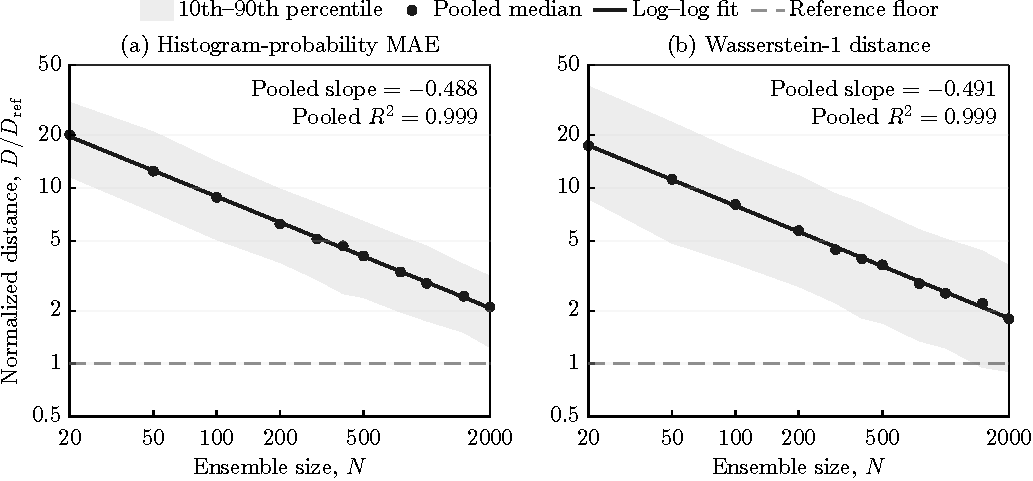
\includegraphics[width=\textwidth]{predict_convergence_reference_floor_summary.pdf}
  \caption{Reference-floor convergence of the PREDICT permeability
  distributions. For each repeated ensemble, the median distance to the three
  reference ensembles is divided by the corresponding empirical reference
  floor. Solid lines and shaded bands show the median and 10th--90th
  percentiles, respectively, over six windows, three permeability components,
  and 30 independent repeats at each sample size. The horizontal dashed line
  marks the empirical reference floor.}
  \label{fig:si-predict-convergence}
\end{figure}

\begin{table}[htbp]
  \centering
  \caption{Summary of the reference-floor convergence assessment. Ratios at
  $N=2000$ pool six windows, three permeability components, and 30 repeats.
  Slopes and $R^2$ values summarize the 18 window--component log--log fits for
  each metric.}
  \label{tab:si-predict-convergence}
  \begin{tabular}{@{}lcccc@{}}
    \toprule
    Metric &
    \multicolumn{2}{c}{Distance/reference floor at $N=2000$} &
    Median slope &
    Median $R^2$ \\
    \cmidrule(lr){2-3}
    & Median & P10--P90 & & \\
    \midrule
    Mean absolute error & 2.10 & 1.24--3.15 & $-0.488$ & 0.993 \\
    Wasserstein-1 distance & 1.80 & 0.90--3.62 & $-0.497$ & 0.988 \\
    \bottomrule
  \end{tabular}
\end{table}

At $N=2000$, the aggregate median discrepancy is within approximately a
factor of two of the empirical large-ensemble floor for both metrics.
Increasing $N$ from 1000 to 2000 reduces the aggregate median normalized
distance by only 27--29\% while doubling the PREDICT cost. Because the fitted
rates indicate continued $N^{-1/2}$ improvement rather than a sharp finite
threshold, $N=2000$ should not be interpreted as exact convergence. Instead,
we select it as a reproducible diminishing-returns compromise that
substantially stabilizes the empirical distributions while keeping subsequent
production-scale PREDICT calculations computationally feasible.

% !TEX root = ../supporting_information.tex

\SISection{Physics-based upscaling of local fault properties}
\label{sec:si-local-fault-property-upscaling}

\SISubsection{Exact realization replay}

Every selected library row stores the original realization identifier,
PREDICT random seed, checkpoint hash, code commit, and method-configuration
hash. Replay uses this provenance record to reconstruct the selected
fine-scale parent units, clay-smear occupancy, porosity, and permeability
fields without archiving every original fine-scale realization. The replayed
effective permeability must agree with the frozen library value within the
validated numerical-equivalence tolerance, while the realization identifier,
seed, code and configuration hashes, and discrete material architecture must
match exactly. A failed check stops downstream upscaling for that fault
element rather than silently substituting another realization.

\todo{Report the final numerical-equivalence tolerance, checkpoint schema,
software versions, and replay-validation coverage across all selected
realizations.}

\SISubsection{Effective permeability and porosity}

Effective permeability is computed with the flow-based PREDICT upscaling
calculation, which applies pressure differences to the replayed fine-scale
fault core and obtains the directional flux responses. Effective porosity is
the pore-volume-weighted average of the fine-cell porosities. Permeability and
porosity are linked to the same replayed realization and are never assembled
from different source rows.

PREDICT reports the permeability tensor in its local fault coordinate system.
Before reservoir export, the tensor is mapped to reservoir-grid coordinates
using
\begin{equation}
  \mathbf{K}_{\mathrm{res}} =
  \mathbf{R}\mathbf{K}_{\mathrm{local}}\mathbf{R}^{\mathsf T},
  \label{eq:si-tensor-rotation}
\end{equation}
where $\mathbf{R}$ contains the local fault-normal, strike, and dip directions
expressed in reservoir coordinates. Exported files retain the local tensor,
rotation metadata, transformed reservoir tensor, component order, and units.
This explicit transformation prevents local $k_{xx}$, $k_{yy}$, and $k_{zz}$
from being interpreted directly as reservoir-grid components.

\todo{State the final local-axis convention, give the explicit rotation
matrix, document the permeability-unit conversion, and report tensor-
transformation validation against the downstream importer.}

\SISubsection{Capillary-pressure upscaling}

Capillary-pressure curves are upscaled by connected invasion percolation on
the replayed fine grid. Local entry pressures are obtained by scaling the
reference material relations with the corresponding fine-cell permeability
and porosity. At each imposed invasion threshold, the connected invaded pore
volume determines the bulk gas saturation. Continuing the invasion sequence
therefore produces both the effective drainage curve and its native maximum
gas-saturation endpoint; the effective irreducible water saturation is one
minus that endpoint.

The production reservoir input retains a separate full-slice capillary-
pressure curve for every one of the 522 fault elements. This representation
preserves along-strike variation in entry pressure, curve shape, and
saturation endpoint. An entry-pressure-branch-medoid representation is
retained only as a documented sensitivity option and is not used for the
production cases described in the main text.

\todo{Provide the reference material curves, Leverett-scaling relation,
invasion boundary condition, connectivity convention, threshold sequence,
and numerical interpolation used for reservoir export.}

\SISubsection{Relative-permeability upscaling}

Dynamic relative-permeability upscaling solves the validated fine-grid flow
problem for an actual replayed slice. For each throw window, the representative
slice is selected as the medoid of the effective irreducible-water-saturation
values obtained from the 87 capillary-pressure upscalings. The resulting gas
and water relative-permeability curve shapes are then mapped to the physical
saturation endpoints of the associated capillary-pressure regions. This
reduces the number of dynamic calculations while preserving the slice-
specific capillary endpoints required for reservoir simulation.

The robust dynamic solver uses internally controlled time stepping and the
validated AMGCL linear solver where supported. The workflow disallows
along-strike grid collapse and representative-slice substitution during the
capillary-pressure calculations. Relative-permeability curves must be
monotonic in the expected direction, remain within $[0,1]$, and terminate at
endpoints consistent with their assigned capillary-pressure regions.

\todo{Describe the fine-grid flow equations, phase properties, boundary and
initial conditions, saturation-state schedule, convergence criteria,
representative-slice medoid calculation, and endpoint-mapping equations.}

\SISubsection{Reservoir-ready consistency checks}

Each reservoir-ready property file is checked for complete $6\times87$
coverage, finite positive permeability, valid porosity, monotonic capillary-
pressure curves, physical relative-permeability bounds, and matching
saturation endpoints. The companion stratigraphy file must have the same
geology identifier and compatible content hash. Additional checks verify the
permeability units, local-to-reservoir tensor transformation, saturation-
region lookup tables, realization provenance, and one-to-one mapping between
the sampling manifest and replayed properties. Export proceeds only after all
checks pass.

\todo{Tabulate every acceptance criterion and report validation coverage for
the complete production dataset.}

% !TEX root = ../supporting_information.tex

\SISection{Construction of full-fault property fields}
\label{sec:si-full-fault-sampling}

\SISubsection{PREDICT library validation}

Each geology-window library contains 2,000 accepted realizations and stores the
joint $(k_{xx},k_{yy},k_{zz})$ vector, original realization identifier,
PREDICT seed, checkpoint hash, code commit, and method-configuration hash.
Automated validation requires complete finite positive permeability values,
unique and replayable provenance records, and a consistent component order.
\todo{Tabulate the frozen library schema and report validation coverage for all
$162\times6$ libraries.}

\SISubsection{Conditionally independent full-fault construction}

Let $\widehat P_{g,w}$ denote the empirical 2,000-member PREDICT library for
geology $g$ and throw window $w$. For stochastic full-fault realization $r$,
the property source assigned to along-strike slice $s$ is sampled as
\begin{equation}
  \boldsymbol{\theta}_{g,w,s,r}
  \sim \widehat P_{g,w},
  \qquad w=1,\ldots,6,\quad s=1,\ldots,87,
  \label{eq:si-conditional-full-fault-sampling}
\end{equation}
where $\boldsymbol{\theta}$ identifies one actual PREDICT realization and
links it to its internally consistent
$(\mathbf{K},\phi,P_c,k_r)$ properties. Sampling is uniform with replacement
and conditionally independent across windows, slices, and stochastic
replicates after conditioning on geology and throw window. This construction
does not infer cross-window correlation or claim that the physical fault is
spatially independent. It deliberately avoids imposing a full-fault
covariance model that is unsupported by the window-by-window PREDICT output.

Every geology uses the same Phase-1 design: 12 stochastic full-distribution
fields, one deterministic full-distribution-medoid field, and coherent low-
and high-state medoid fields. Phase 1 therefore contains
$162\times15=2{,}430$ field-scale cases. Only the 12 stochastic fields per
geology enter empirical probabilities, conditional distributions, or global
variance decompositions. The three deterministic fields are diagnostic
benchmarks and carry no probability weight.

\SISubsection{Full-distribution and state-library medoids}

For log-permeability vector
\begin{equation}
  \mathbf{y}_i =
  (\log_{10}k_{xx,i},\log_{10}k_{yy,i},\log_{10}k_{zz,i}),
\end{equation}
the full-distribution medoid is
\begin{equation}
  i_{\mathrm{full}}=
  \arg\min_i\sum_{j=1}^{2000}\lVert\mathbf{y}_i-\mathbf{y}_j\rVert_2.
  \label{eq:si-full-medoid}
\end{equation}
Ties are broken using the smallest original realization identifier. The
result is therefore an actual joint PREDICT realization rather than a
synthetic component-wise median.

Low and high state libraries retain 20\% of each window library. Joint samples
are clustered in physical three-dimensional $\log_{10}(k)$ space with
$k$-medoids over $K=1,\ldots,5$. A multi-cluster solution must have at least
5\% of samples in every cluster and a mean silhouette of at least 0.25.
Clusters are ordered by the median joint rank score
\begin{equation}
  r_{\mathrm{joint}}^{(m)} =
  \frac{r_{xx}^{(m)}+r_{yy}^{(m)}+r_{zz}^{(m)}}{3}.
\end{equation}
Complete extreme clusters are retained where possible, and the boundary
cluster is truncated by joint-rank order to obtain exactly 400 samples. The
low/high benchmark realization is the medoid of the final 400-member library,
not necessarily the medoid of one constituent cluster.

\SISubsection{Deterministic full-fault manifests}

Every case manifest contains 522 rows, one for each window-slice element. For
an independent case, one source row is sampled uniformly with replacement from
the complete 2,000-member library of the corresponding window. Seeds are
derived from a stable hash of the base seed, geology identifier, phase, case
type, replicate identifier, and window identifier. Consequently, manifests
are byte-reproducible and independent of parallel execution order.

The representative benchmark assigns the full-distribution medoid of each
window to all 87 slices in that window. The low- and high-state stress
benchmarks analogously assign their state-library medoids, producing coherent
fault-wide low and high fields. These fields test representative and stress
behavior; they are not interpreted as bounds or percentiles. Each manifest
row explicitly records whether it belongs to the probabilistic ensemble, a
representative benchmark, or a stress benchmark. \todo{Provide the complete
manifest schema, seed-hash algorithm, and case-identifier table.}

\SISubsection{Sampling-fidelity and independence checks}

For each geology-window pair, the 12 Phase-1 independent fields provide
$12\times87=1{,}044$ draws. Their component-wise Wasserstein distances and
joint energy distance from the 2,000-member source library are compared with a
reference distribution obtained from synthetic 1,044-member samples. Pairwise
rank correlations between windows at matching slice indices are likewise
compared with simulations under independence. These tests verify marginal
fidelity and detect accidental coupling from shared streams or rank matching;
they do not establish geological independence. \todo{Report acceptance
intervals and results for all production manifests.}

% !TEX root = ../supporting_information.tex

\SISection{Field-scale reservoir simulation of geologic
\texorpdfstring{\coTwo{}}{CO2} storage}
\label{sec:si-field-scale-reservoir-simulation}

\SISubsection{Reservoir model and simulation setup}

The field-scale model contains approximately two million active cells and
represents megatonne-scale \coTwo{} injection into the offshore Texas storage
interval followed by migration and containment over 1,000 years. JutulDarcy
solves the multiphase flow problem. Each realization preserves the common
reservoir geometry and operating conditions while replacing the geology-
specific stratigraphy and the spatially variable fault permeability,
porosity, capillary-pressure functions, and relative-permeability functions.

\todo{Document the JutulDarcy version, grid and fluid model, injection
schedule, well controls, and boundary and initial conditions.}

\SISubsection{Reservoir-input validation}

Before model construction, the importer verifies that the fault-property and
stratigraphy files share the same geology identifier, design metadata, and
compatible hashes. It then checks complete six-window by 87-slice coverage,
permeability units and coordinate convention, porosity bounds, capillary-
pressure and relative-permeability region indices, and consistency of the
native saturation endpoints.

\SISubsection{Numerical verification and restart procedures}

A case is accepted for analysis only after the simulation reaches the
requested final time and passes the prescribed mass-balance and output-
integrity checks.

\todo{Document the nonlinear and linear solvers, timestep controls, restart
procedure, mass-balance tolerance, five saved output times, failed-case
recovery rules, and final validation results.}

% !TEX root = ../supporting_information.tex

\SISection{Uncertainty quantification of
\texorpdfstring{\coTwo{}}{CO2} migration and containment}
\label{sec:si-migration-containment-uq}

\SISubsection{Quantities of interest and outcome classes}

Primary containment responses quantify whether \coTwo{} enters the top seal
and the corresponding mass fraction. The primary migration response is the
maximum upward distance reached by \coTwo{} relative to the injection
interval. Secondary responses include the fractions of injected \coTwo{}
retained in the storage reservoir, entering the modeled fault and overburden,
and partitioned between dissolved and free phases. All mass fractions use a
common injected-mass denominator and are evaluated at prespecified output
times.

Outcome classes distinguish consistent containment, localized fault entry,
substantial upward migration, and top-seal or overburden interaction. Their
spatial masks and numerical thresholds are defined before inspecting the
complete ensemble so that classification does not adapt to the observed
results. \todo{Provide the final storage-reservoir, fault, top-seal, and
overburden masks; injected-mass denominator; free and dissolved component
accounting; maximum-migration calculation; numerical entry tolerances;
evaluation times; and class thresholds.}

\SISubsection{Design-based geologic effects}

The common 12 independent realizations per geology form a balanced nested
design. For continuous response $Q_{g,r}$, geologic effects are estimated from
the four prescribed factors and selected interactions with realizations nested
within geology. Effects are interpreted over the uniform scenario design, not
as sensitivities weighted by field occurrence probabilities. Entry quantities
with a point mass at zero are separated into an occurrence model and a
conditional-magnitude model. \todo{State the final model form, contrasts,
standardization, uncertainty intervals, and interaction-selection rule.}

For each geology, the 12 stochastic realizations also estimate the conditional
median, robust spread, empirical outcome frequencies, and empirical CDFs. The
medoid and low/high benchmark cases are excluded from these estimators. This
separation prevents deterministic diagnostic fields from being counted as
random draws from the conditional fault-property distribution.

\SISubsection{Between- and within-geology contributions}

Let $\bar Q_g$ and $s_g^2$ denote the sample mean and variance among the 12
independent realizations for geology $g$. With $G=162$, the average
within-geology contribution is estimated as
\begin{equation}
  \widehat V_{\mathrm{within}}
  =\frac{1}{G}\sum_{g=1}^{G}s_g^2.
\end{equation}
The variance among $\bar Q_g$ includes finite-replicate noise, so the
between-geology design contribution is estimated as
\begin{equation}
  \widehat V_{\mathrm{between}}
  =\max\left[0,
  \operatorname{Var}_g(\bar Q_g)
  -\frac{1}{G}\sum_{g=1}^{G}\frac{s_g^2}{12}\right].
\end{equation}
Normalized contributions divide each quantity by their sum. Robust spreads
and outcome-class disagreement accompany this variance summary when responses
are non-Gaussian, zero-inflated, or multimodal.

\SISubsection{Targeted enrichment and confirmatory analysis}

Phase-1 results nominate geologies using prespecified criteria: more than one
outcome class, large robust conditional spread, medoid--ensemble disagreement,
stress benchmarks on opposite sides of a physical threshold, and coverage of
the geologic design space. Twelve geologies receive 20 new independent
realizations. The six that remain most realization sensitive receive 40
further realizations. Selection statistics use only earlier simulations;
newly added simulations evaluate whether the apparent sensitivity persists.
\todo{Report the exact thresholds, selected geology identifiers, normalized
geologic-space coverage, and all selection decisions.}

\SISubsection{Representative and stress benchmark analyses}

For each geology, representative-fault performance is quantified by the
difference between the medoid result and the stochastic median, the medoid's
position in the empirical stochastic CDF, and agreement with the majority
outcome class. Low/high benchmarks are compared as coherent state stresses but
are excluded from empirical CDFs, variance contributions, and outcome
probabilities. \todo{Add threshold-sensitivity analyses and complete benchmark
results for all quantities of interest.}


\bibliography{references}

\end{document}
